
\chapter{Implementación}
\label{chap:implementación}

Una vez descrito el diseño del sistema, llegamos a la etapa de implementación. Uno de los objetivos del trabajo era verificar que la arquitectura elegida era viable. Para ello, optamos por implementar un sistema autoadaptativo muy básico. Tanto el diseño como la implementación se desarrollaron de forma incremental. Gracias a esto, el diseño fue evolucionando según detectábamos nuevas necesidades o problemas que no resolvía nuestra arquitectura.

En este capitulo describiremos la implementación de los microservicios del nivel de conocimiento de conocimiento y del bucle. Dejaremos para más adelante, en el capitulo \ref{chap:caso_estudio}, la descripción de la implementación del nivel de solución y sistema manejado. En este capitulo ofrecemos una vista más concreta de la implementación, y las tecnologías empleadas. En el otro describiremos cómo encaja todo a nivel general y veremos cómo opera.

La implementación se llevo a cabo en 4 hitos distintos, cada uno correspondiente a una etapa distinta del bucle:

\begin{itemize}
  \item \textbf{Hito 1 - Servicio de monitorización y conocimiento}
  \item \textbf{Hito 2 - Servicio de análisis y reglas}
  \item \textbf{Hito 3 - Planificador}
  \item \textbf{Hito 4 - Ejecutor y efectores}
\end{itemize}

\section{Servicio de monitorización y conocimiento}

En esta primera etapa desarrollamos el proceso de monitorización. Este abarca desde que la sonda realiza sus mediciones hasta que se graban en el conocimiento. Esto implicó implementar varios componentes: las sondas y monitores del caso de estudio (capitulo \ref{chap:caso_estudio}), el componente de monitorización del bucle MAPE-K y la base de conocimiento.

%% TODO: dotnet logo?
Para su desarrollo se optó por el lenguaje C\# y el \foreign{english}{framework} ASP.NET\footnote{Página oficial: \url{https://docs.microsoft.com/en-us/aspnet/core/introduction-to-aspnet-core}}. Este \emph{framework} es específico para implementar servidores web de la plataforma .NET de Microsoft. Lo elegimos porque ya contábamos con experiencia de desarrollo en esta plataforma. Además de que soporta los principales sistemas operativos (Windows, Linux y Mac).

\subsection{Peticiones síncronas}

En este hito también se prototiparon los conectores para peticiones síncronas. Aquellos servicios que las soporten expondrán \foreign{english}{endpoints} HTTP. Por ejemplo, el servicio de conocimiento expone aquellos que permiten recuperar o modificar propiedades de adaptación.  En el fragmento \ref{ls:csharp-get} ya mostramos un ejemplo de su implementación.

Gracias al uso de la librería \emph{Swashbuckle.AspNetCore}\footnote{Página oficial: \url{https://github.com/domaindrivendev/Swashbuckle.AspNetCore}}, pudimos generar su especificación en el estándar OpenAPI. Esto nos aportó dos cosas: una interfaz de usuario para interactuar con la API y la posibilidad de generar el API client.

Hablemos primero sobre la interfaz de usuario. La librería añade a nuestro servicio el \foreign{english}{endpoint} \texttt{/swagger}. Accediendo a esta ruta, se nos servirá una interfaz con un listado de todas las operaciones que ofrece la API (figura \ref{fig:swagger-knowledge-ui}). De cada petición nos muestra su documentación (la que añadimos en el código) y sus parámetros. Incluso nos permite ejecutarlas. De esta forma, los usuarios pueden investigar qué ofrece la API y hacer pruebas.

\begin{figure}[htb]
  \centering
  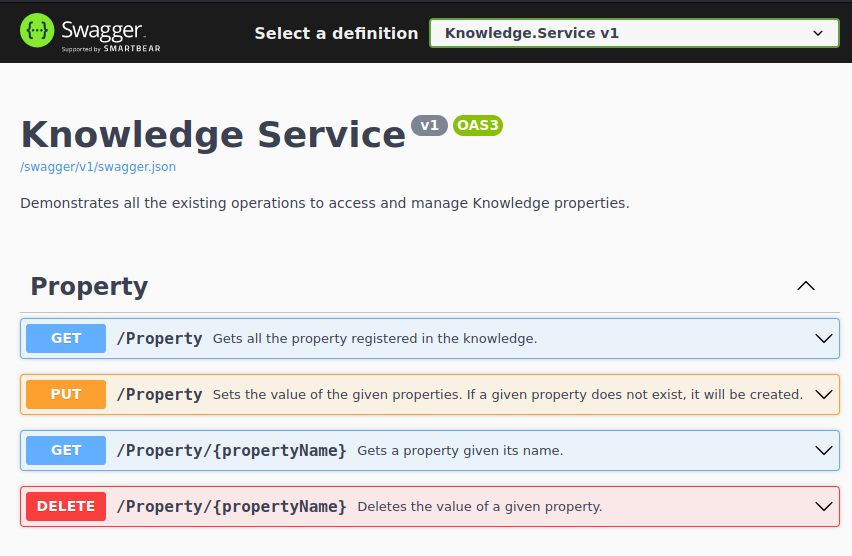
\includegraphics[scale=1.5]{cap_implementacion/images/swagger-knowledge-ui}
  \caption{Interfaz de usuario ofrecida por Swagger para el servicio de conocimiento. Se genera a partir de las especificación OpenAPI.}
  \label{fig:swagger-knowledge-ui}
\end{figure}

Por otro lado, también nos permite generar el API Client. Como comentamos en la sección \ref{chap:OpenAPI} de OpenAPI, tenemos gran variedad de generadores de código a nuestra disposición. Nosotros optamos por la librería \texttt{OpenAPI.Generator}\footnote{Página del proyecto: \url{https://github.com/OpenAPITools/openapi-generator}}. En concreto, el generador de código de \verb|C#|. Usándolo pudimos generar una librería que permite contactar con nuestro servicio, sin necesidad de implementar mucho código. Por ejemplo, el componente de monitorización del bucle contacta a través de un API Client generado.

\subsection{Componentes: Módulos de monitorización y conocimiento}

El módulo del conocimiento es un servicio muy sencillo. Ofrece operaciones de lectura y escritura sobre las propiedades de adaptación y las claves de configuración de servicios manejados. Para el prototipo estas se almacenan en diccionarios en memoria. Cuando el servicio se reinicie, los valores se perderán.

Por encima de este, tenemos el servicio de monitorización. En nuestra implementación, actúa como intermediario entre los monitores de la solución y el conocimiento. También se trata de un servicio sencillo. Ofrece operaciones útiles para los monitores de la solución: lectura de propiedades del conocimiento y otras para que los monitores reporten sus mediciones. De esta forma, los monitores de solución podrán informarse a partir del conocimiento para determinar si una medición es válida o no.

\textcolor{red}{¿Añadir ejemplos de código? ¿Describir los componentes implementados? ¿Debería unificarse con el capítulo de implementación del caso de estudio?}

\section{Servicio de análisis y reglas}
\label{sec:implementacion-modulo-reglas}

En el segundo hito, acordamos implementar la evaluación de reglas de adaptación. Esto requería de implementar el servicio de análisis del bucle MAPE-K y los servicios de reglas de la solución. En este hito empezamos a plantearnos el diseño de las comunicaciones ascendentes: las notificaciones. Con ellas, evitaríamos que se los componentes se acoplaran a la capa superior.

\subsection{Notificaciones}

%% TODO: Logo RabbitMQ?
Comenzaremos describiendo el desarrollo de las notificaciones. Como ya se describió en la sección \ref{sec:notificaciones}, este componente se implementó mediante un \foreign{english}{broker} de mensajería. Elegimos \texttt{RabbitMQ}\footnote{Página oficial: \url{https://www.rabbitmq.com/}}, uno ''sencillo'' y ampliamente utilizado. \cite{newmanBuildingMicroservicesDesigning2021} Con él pudimos  implementar los dos patrones de comunicación que necesitamos: las notificaciones y las peticiones asíncronas.

Para implementar nuestro conector, utilizamos una librería llamada \texttt{Rebus}\footnote{Página oficial: \url{https://github.com/rebus-org/Rebus}}. Esta nos permite interactuar con un bus, abstrayéndonos de la tecnología concreta utilizada para la comunicación. Así, podríamos cambiar de tecnología de transporte en cualquier momento por otra que se ajuste más a nuestros requisitos.

Finalmente, para desacoplar la funcionalidad de de la publicación y consumición de mensajes del bus, empleamos \texttt{MediatR}\footnote{Página oficial: \url{https://github.com/jbogard/MediatR}}. Esta librería implementa el patrón mediador. Nos permite propagar mensajes dentro de un proceso. En nuestro caso, los eventos. Ni el emisor ni el receptor requieren tener referencias del otro. Es similar a un \foreign{english}{broker} de mensajería, pero funcionando interproceso.

Ahora nos centraremos en la comunicación entre el módulo de conocimiento y el servicio de análisis. Una vez se confirma la escritura de una propiedad o configuración en el conocimiento, este debe notificar a los servicios en la capa superior. Para ello, comienza propagando internamente un \textbf{evento de integración} (línea 11 del fragmento \ref{ls:knowledge-set-property}) mediante el mediador.


\begin{lstlisting}[language={[Sharp]C},caption={Implementación del método que asigna valor a una propiedad. Muestra un ejemplo de propagación interna de eventos de integración.},captionpos=b, label=ls:knowledge-set-property]
private async Task SetProperty(SetPropertyDTO propertyDto)
{
    var newValue = new()
    {
        Value = propertyDto.Value,
        LastModification = DateTime.UtcNow,
    };

    properties.AddOrUpdate(propertyDto.Name, newValue, (_, _) => newValue);

    await _mediator.Send(
      new PropertyChangedIntegrationEvent(propertyDto.Name));
}

\end{lstlisting}

El mediador determinará que nuestro componente publicador es el destinatario de este evento. Lo hace en base a las interfaces que implementa (linea 2 del fragmento \ref{ls:knowledge-property-changed-publisher}). Este componente publica el evento en el bus de mensajería (línea 15). Rebus, en base a la configuración del servicio, lo enviará a nuestra instancia de \texttt{RabbitMQ} y lo publicará en el \foreign{english}{exchange} correspondiente. Todos los suscriptores ubicados en la capa superior lo recibirán en su cola.

\begin{lstlisting}[language={[Sharp]C},caption={El publicador de eventos captura el evento de integración y lo publica en el bus.},captionpos=b, label=ls:knowledge-property-changed-publisher]
public class PropertyChangedIntegrationEventPublisher
  : IIntegrationEventPublisher<PropertyChangedIntegrationEvent>
{
  private readonly IBus _bus;

  public PropertyChangedIntegrationEventPublisher(IBus bus)
  {
      _bus = bus;
  }

  public async Task<Unit> Handle(
      PropertyChangedIntegrationEvent notification,
      CancellationToken cancellationToken)
  {
      await _bus.Publish(notification);

      return Unit.Value;
  }
}
\end{lstlisting}

Finalmente, en el servicio de análisis, tenemos el componente consumidor (fragmento \ref{ls:analysis-property-changed-consumer}). \texttt{Rebus} obtendrá el evento de la cola de mensajería y se lo pasará a nuestro consumidor. Este lo recibirá y lo propagará internamente en el servicio (línea 20). Todos los manejadores (\foreign{english}{handlers}) del evento lo recibirán y podrán tratarlo.

\begin{lstlisting}[language={[Sharp]C},caption={El consumidor recibe el evento de integración del bus y lo propaga internamente. Todos los manejadores de este evento lo recibirán.},captionpos=b, label=ls:analysis-property-changed-consumer]
public class PropertyChangedIntegrationEventConsumer
  : IIntegrationEventConsumer<PropertyChangedIntegrationEvent>
{
  private readonly IMediator _mediator;

  public PropertyChangedIntegrationEventConsumer(IMediator mediator)
  {
      _mediator = mediator;
  }

  public async Task Handle(PropertyChangedIntegrationEvent message)
  {
      await _mediator.Publish(message);
  }
}
\end{lstlisting}

\subsection{Componentes: Servicio de análisis y módulos de reglas}

En cuanto a la implementación del módulo de análisis, este realmente no cuenta tampoco con mucha lógica. Participa como intermediario entre el conocimiento y los servicios de reglas. Como hemos visto, recibe los eventos de cambios en las propiedades y los propaga a la capa superior. Ofrece operaciones de solo lecturas de propiedades y configuración del conocimiento. Así, limitamos las escrituras por parte de las reglas.

Se podría considerar que este servicio ha quedado anémico \textcolor{red}{referencia}. En trabajos posteriores, este servicio podría ampliarse añadiendo autenticación y autorización. Así, se podría evitar que servicios no autorizados accedan a sus operaciones o soliciten adaptaciones maliciosas.

Respecto a la implementación de los módulos de reglas, ofrecemos una implementación de referencia. Aunque como estos se encuentran en nivel de la solución, el desarrollador es libre de elegir si implementarla u optar por otra distinta.

En el fragmento \ref{ls:adaption-rule-base} mostramos la clase base de las reglas de adaptación. Vemos que esta clase está suscrita a los eventos de integración de cambio de propiedad de adaptación y cambio en la configuración del sistema (lineas 2-3). Cuando el consumidor capture uno de estos eventos, lo propagará internamente y todas las reglas afectadas lo capturarán.

Esta clase base se desarrolló siguiendo el patrón plantilla (o \foreign{english}{template})\footnote{\url{https://refactoring.guru/design-patterns/template-method}}. Define un método que evalúa la condición de la regla (\texttt{EvaluateCondition}) y, si esta se cumple, la ejecuta (\texttt{Execute}). Las reglas que hereden de esta deberán de implementar ambos métodos.

\begin{lstlisting}[language={[Sharp]C},caption={Clase base para implementar reglas de adaptación. Se evalúa la condición, y si esta se cumple, se ejecuta.},captionpos=b, label=ls:adaption-rule-base]
public abstract class AdaptionRuleBase
    : IIntegrationEventHandler<PropertyChangedIntegrationEvent>,
      IIntegrationEventHandler<ConfigurationChangedIntegrationEvent>
{
    // ..

    private async Task Handle()
    {
        try
        {
            if (await EvaluateCondition())
            {
                await Execute();
            }
        }
        catch (Exception e)
        {
            _diagnostics.RuleEvaluationError(_ruleName, e);

            throw;
        }
    }

    protected abstract Task<bool> EvaluateCondition();

    protected abstract Task Execute();

    // ..
}
\end{lstlisting}

Respecto a las suscripciones, las herederas deberán indicar de qué propiedades o claves de configuración dependen. En base a ellas, deberemos suscribirnos a las notificaciones que emite el módulo de análisis. Para ello, hemos implementado una serie de atributos que permiten declarar estas dependencias.

En el fragmento \ref{ls:adaption-rule-dependencies} mostramos un ejemplo. En la línea 1 tenemos el atributo que describe las dependencias con la propiedad de adaptación \texttt{Temperature}. Por otro lado, en las líneas 2-5 tenemos la declaración de dependencias con dos claves de configuración del servicio \texttt{Climatisation.AirConditioner}: \texttt{TargetTemperature} y \texttt{Mode}.

\begin{lstlisting}[language={[Sharp]C},caption={Las reglas declaran sus dependencias sobre propiedades de adaptación usando atributos. Estos se utilizarán para las suscripciones a los temas de los eventos.},captionpos=b, label=ls:adaption-rule-dependencies]
[RuleKnowledgePropertyDependency(ClimatisationConstants.Property.Temperature)]
[RuleServiceConfigurationDependency(
    ClimatisationAirConditionerConstants.AppName,
    ClimatisationAirConditionerConstants.Configuration.TargetTemperature,
    ClimatisationAirConditionerConstants.Configuration.Mode)]
public class DisableAirConditionerWhenCoolingAndTargetTemperatureAchievedAdaptionRule
  : AdaptionRuleBase
{
    // ...
}
\end{lstlisting}

Para suscribirnos a las notificaciones de cambio de las dependencias de las reglas utilizaremos la \textbf{reflexión}: analizaremos el ensamblado del servicio buscando todas las reglas y obtendremos los valores de sus atributos. En base a ellos, nos suscribiremos a los \foreign{english}{topics} en el \foreign{english}{broker} de mensajería.

\begin{lstlisting}[language={[Sharp]C},caption={Para suscribirnos a los \foreign{english}{topics} de las notificaciones obtenemos las dependencias de las reglas mediante reflexión},captionpos=b, label=ls:rules-registration]
public static IServiceCollection AddAdaptionLoopAnalysisServices(
  this IServiceCollection services,
  IConfiguration configuration,
  Assembly rulesAssembly)
{
    // ...

    services.AddBus(
        configuration,
        rulesAssembly,
        registerSubscriptions: async bus =>
        {
            var subscriptions = GetRulesBusTopicNames(rulesAssembly);

            foreach (var subscription in subscriptions)
            {
                await bus.Advanced.Topics.Subscribe(subscription);
            }
        });

    return services;
}
\end{lstlisting}

\section{Planificador}

En el tercer hito implementamos las peticiones de cambio de las reglas y el servicio de planificación. Aquí surge también la necesidad de un tercer patrón de comunicación: las peticiones asíncronas.

\subsection{Peticiones asíncronas}

Continuando por donde nos quedamos, una vez se evalúa la condición de la regla y esta estima que debe ejecutarse, necesitamos un mecanismo para solicitar cambios en la configuración del sistema. En el cuerpo de la regla se solicitarán cambios a la configuración actual del sistema en base a los síntomas que haya detectado la regla. En el fragmento \ref{ls:change-request-builder} mostramos un ejemplo de esta solicitud de cambio. Para un síntoma determinado, \texttt{TemperatureGreaterThanHotThreshold} (línea 6), requerimos que el servicio \texttt{Climatisation.AirConditionerService} esté presente (lineas 7-10) con la configuración \texttt{Mode} con el valor \texttt{Cooling} (lineas 11-13).

\begin{lstlisting}[language={[Sharp]C},caption={Implementación de la misma petición siguiendo el patrón \emph{builder}.},captionpos=b, label=ls:change-request-builder]
protected override async Task Execute()
{
  await _systemService.RequestConfigurationChange(changeRequest =>
  {
    changeRequest
      .ForSymptom(TemperatureGreaterThanHotThreshold)
      .WithService(ClimatisationAirConditionerConstants.AppName, service =>
      {
        service
          .MustBePresent()
          .WithParameter(
            ClimatisationAirConditionerConstants.Configuration.Mode,
            AirConditioningMode.Cooling.ToString());
      });
  });
}
\end{lstlisting}

Las reglas comunicarán esta solicitud de cambio al módulo de análisis. Esta solicitud de cambio deberá comunicársela al módulo de análisis, que la redirigirá al planificador. Este deberá generar un \textbf{plan de cambio} a partir de las solicitudes.

Para redirigir esta petición de cambio, usaremos las peticiones asíncronas. Su implementación es muy similar a la de las notificaciones, explicada en detalle en el apartado anterior. La única diferencia radica en la cardinalidad de la comunicación: el módulo de análisis publicará el mensaje directamente en la cola de trabajo, en lugar de publicarlo en un exchange para que lo reciba cualquier subscriptor. Entonces, sólo cambia la implementación del publicador. En la línea 14 del fragmento \ref{ls:request-publisher} vemos que el mensaje se enruta directamente a la cola \texttt{PlanningServiceQueue}.

\begin{lstlisting}[language={[Sharp]C},caption={Para suscribirnos a los \foreign{english}{topics} de las notificaciones obtenemos las dependencias de las reglas mediante reflexión},captionpos=b, label=ls:request-publisher]
public class SystemConfigurationChangeRequestPublisher
  : IRequestPublisher<SystemConfigurationChangeRequest>
  where TRequest : Request
{
  public SystemConfigurationChangeRequestPublisher(IBus bus)
  {
      _bus = bus;
  }

  public async Task<Unit> Handle(
      SystemConfigurationChangeRequest request,
      CancellationToken cancellationToken)
  {
      await _bus.Advanced.Routing.Send(
          AdaptionLoopPlanningConstants.Queues.PlanningServiceQueue,
          request);

      return Unit.Value;
  }
}
  \end{lstlisting}

El resto de la implementación será muy similar. Solo cambiará las interfaces que debamos implementar para cada tipo de componente (\texttt{IRequestConsumer} en lugar de \texttt{IIntegrationEventConsumer}, etc.).

\subsection{Componentes: Servicio de planificación}

El planificador recibirá esta petición de cambio y deberá elaborar un plan de adaptación. Para ello, verificará que el plan de cambio es viable. En nuestro prototipo, para reducir el ámbito del proyecto, nos limitamos a comprobar que la configuración sea distinta a la configuración actual. Si el sistema ya se encuentra en el estado solicitado, el plan de cambio se queda vacío y no se propaga.

Para ello, el servicio de planificación compara la configuración actual con la solicitada, y añade al plan de adaptación las \textbf{acciones de adaptación} requeridas para alcanzar el estado deseado. Ya comentamos que los operadores arquitectónicos con los que operaremos serán del ámbito de los microservicios: activar servicio, eliminar servicio, vincular servicios, desvincularlos y cambiar su configuración.

Por ejemplo, un plan de adaptación para la regla evaluada anteriormente sería:

\begin{lstlisting}[language=python,caption={Plan de adaptación generado. Solo contiene una acción de adaptación: cambiar la configuración \texttt{Mode} del servicio \texttt{AirConditioner}.},captionpos=b, label=ls:adaption-change-plan]
{
  "ChangePlan": {
    "Timestamp": "2022-07-09T09:53:01.1868834Z",
    "Actions":
    [
      {
        "Type": 3, // Set Parameter
        "ServiceName": "Climatisation.AirConditioner.Service",
        "PropertyName": "Mode",
        "PropertyValue": "Cooling"
      }
    ]
  },
  "Symptoms":
  [
    {
      "Name": "temperature-lesser-than-cold-threshold",
      "Value": "true"
    }
  ]
}
\end{lstlisting}

\section{Ejecutor y efectores}

En el hito final implementamos el módulo ejecutor y los efectores. Este módulo recibirá el plan de adaptación del planificador. A partir de este, deberá distribuir las acciones de adaptación que contiene entre sus servicios de efectores.

Para transmitirle el plan de adaptación del planificador al ejecutor, volvemos a recurrir a las peticiones asíncronas. De forma similar al servicio de análisis y el planificador, estos se encuentran en la misma capa. El plan de adaptación que se le pasa como evento de integración es el que ya mostramos en el fragmento \ref{ls:adaption-change-plan}.

Una vez captura la petición, el ejecutor deberá determinar qué servicios debe cambiar, y manipular sus efectores. Para nuestra implementación, simplemente agrupamos las acciones por el nombre del servicio afectado. Las publicaremos como notificaciones usando el nombre del servicio como tema.

Estas notificaciones las capturan los servicios de efectores.
La comunicación entre el módulo de planificación  y el ejecutor. El efector actúa como un traductor del modelo de alto nivel al nivel del sistema: \textcolor{red}{citar paper de garlan} para cada acción de adaptación, deberá determinar cómo ejecutarla en el sistema manejado. Estos servicios son los que manipularán el estado del sistema. Actúan como envoltorios del mismo. La comunicación entre este servicio y el sistema es un tanto especial: dependerá del sistema manejado; de si tenemos control sobre su implementación. Si no es así, tendremos que adaptarnos a la implementación que ofrezca este (HTTP, mensajería...).

Dependiendo de la acción, el efector hará una acción u otra: deplegar un servicio, o eliminarlo, cambiar la configuración, etc.

Continuando con nuestro ejemplo del modo del aire acondicionado, el sistema modificaría la configuración del mismo. Una vez se confime el cambio, si se ha llevado a cabo, se ejecutará actualizará su valor en la base de conocimiento. Dependerá de si el sistema es capaz de hacerlo o debe recaer la responsabilidad en el efector.
